% LOC3X1 Modernization PoC Handbook
\documentclass[11pt]{article}
\usepackage[margin=1in]{geometry}
\usepackage{hyperref}
\usepackage{graphicx}
\usepackage{tikz}
\usetikzlibrary{arrows.meta,positioning,fit}
% Make arrowheads larger (about 5x) using arrows.meta and define a stylish arrow style
\tikzset{>={Latex[length=10mm,width=5mm]},
  flowarrow/.style={->,>=Latex,line width=1.2pt,draw=black!80,line cap=round}
}
\usepackage{booktabs}
\usepackage{array}
\usepackage{caption}
\usepackage{algorithm}
\usepackage{algpseudocode}
\usepackage{xcolor}
\usepackage{listings}

% Styled code boxes for XML-based specs
\lstdefinestyle{codebox}{
  basicstyle=\ttfamily\footnotesize,
  frame=single,
  backgroundcolor=\color{gray!10},
  columns=fullflexible,
  breaklines=true,
}

\hypersetup{
  colorlinks=true,
  linkcolor=blue,
  citecolor=blue,
  urlcolor=blue
}

\title{LOC3X1 Modernization PoC Handbook}
\author{Alberto Hernandez}
\date{\today}

\begin{document}
\maketitle
\begin{abstract}
This handbook explains, from first principles, the technologies and design behind a modernization Proof of Concept (PoC) for the LOC3X1 domain. It covers the client-provided \texttt{Dependencies} folder (WSDL/XSD, mapping specs, BPEL), the modern Spring Boot + Apache Camel implementation, and how mapping, validation, and enrichment combine to produce the final XML output. The content is intended for readers with no prior knowledge of Java, Maven, SOAP, or BPEL, and includes diagrams, tables, and pseudocode to make the logic approachable. References are provided and are clickable. 
\end{abstract}

\tableofcontents

\section{Background and Goals}
\subsection{Problem Context}
The client supplied an authoritative \texttt{Dependencies} folder containing: WSDL (service contracts), XSD (data schemas), mapping specifications (\texttt{.map}), and a BPEL process definition. The modernisation goal is to implement equivalent business logic in a cloud-friendly, maintainable stack, demonstrating correctness by producing deterministic XML output. 

This modernisation effort addresses a fundamental challenge in enterprise software evolution: legacy systems built on vendor-specific orchestration engines and proprietary tooling must be translated into open, portable frameworks that support contemporary development practices—version control, automated testing, continuous integration, and containerised deployment. The client's \texttt{Dependencies} folder represents the complete specification of a location retrieval workflow originally implemented using early-2000s enterprise service bus (ESB) technology. Our task is to preserve the exact business semantics whilst replacing the execution substrate.

\subsection{Level 1: Client Legacy Landscape (Old Technology)}\label{subsec:client-legacy-landscape}
This first level introduces the original code and specifications living in \texttt{CHUBB/Dependencies/}. It explains how contracts (WSDL), schemas (XSD), mapping specifications (\texttt{.map}), and BPEL orchestrations fit together. Understanding these artefacts is essential: they encode not merely technical details but the business logic, data governance rules, and integration contracts that have been validated over years of production use.

\paragraph{Legacy-only Diagram}
\begin{center}
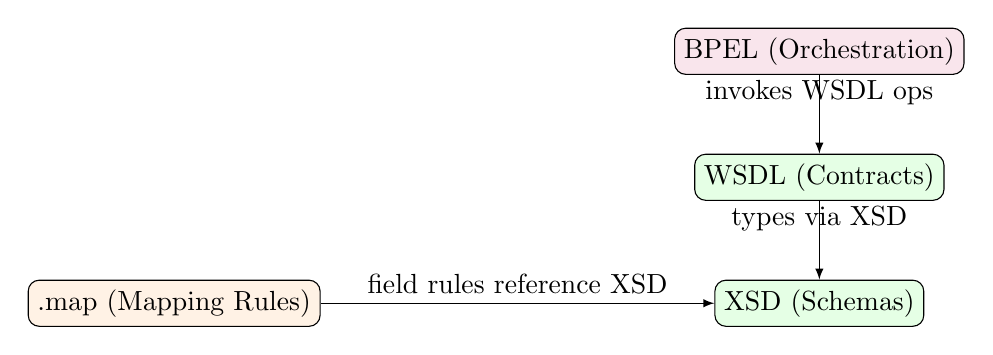
\begin{tikzpicture}[node distance=1.6cm,>=latex]
  % Legacy specs only (without Dependencies node)
  \node (bpel) [draw, rounded corners, fill=purple!10] {BPEL (Orchestration)};
  \node (wsdl) [below of=bpel, draw, rounded corners, fill=green!10] {WSDL (Contracts)};
  \node (xsd)  [below of=wsdl, draw, rounded corners, fill=green!10] {XSD (Schemas)};
  \node (map)  [left=5cm of xsd, draw, rounded corners, fill=orange!10] {.map (Mapping Rules)};
  
  % Relationships amongst legacy assets
  \draw[->] (wsdl) -- node[above]{types via XSD} (xsd);
  \draw[->] (bpel) -- node[above]{invokes WSDL ops} (wsdl);
  \draw[->] (map) -- node[above]{field rules reference XSD} (xsd);
\end{tikzpicture}
\end{center}

\paragraph{Key Concepts for Modern Developers}

Before examining the code samples, it is crucial to understand what each technology accomplishes and why it exists. These are not arbitrary choices; each addresses a specific problem in distributed enterprise systems.

\begin{itemize}
  \item \textbf{WSDL (Web Services Description Language)}: A WSDL document functions as a formal contract between service provider and consumer. It answers three essential questions: \emph{What operations are available?} (e.g., \texttt{GetLocationList}), \emph{What data structures do they accept and return?} (messages with typed parts), and \emph{How do I communicate?} (protocol bindings, typically SOAP over HTTP). If you have encountered OpenAPI (formerly Swagger) specifications for RESTful APIs, WSDL serves an analogous purpose for SOAP-based web services: it provides machine-readable metadata enabling automated client generation, compile-time validation, and runtime introspection. The WSDL vocabulary includes \texttt{types} (data schemas), \texttt{messages} (operation parameters), \texttt{portType} (abstract operations), \texttt{binding} (concrete protocol mapping), and \texttt{service} (network endpoints). For a modern developer, understanding WSDL is essential because many enterprise systems still expose SOAP interfaces, and tools like Apache CXF or JAX-WS can generate Java or Python client code directly from WSDL, eliminating manual serialisation logic.

  \vspace{0.5em}
  \noindent\fbox{\parbox{0.95\textwidth}{%
  \textbf{\textcolor{red}{Step 1: Generate stubs from WSDL (wsdl2java/wsimport)}}\\
  \emph{Implemented}: WSDLs in \texttt{CHUBB/Dependencies/LocationRetrievalLOC3X1*/} produce client stubs packaged in \texttt{libs/soap-clients-0.0.1-SNAPSHOT.jar}; these types are referenced by routes/controllers (e.g., demo client at \texttt{GET /api/index}).\\
  \emph{Enhance}: Move stub generation into the build (Maven/Gradle) with locked plugin versions, generate sources to \texttt{target/generated-sources}, and include smoke tests that call mocked SOAP endpoints to ensure stubs align with WSDL changes.
  }}
  \vspace{0.5em}

  \item \textbf{XSD (XML Schema Definition)}: An XSD file defines the permissible structure, data types, constraints, and cardinality of XML documents. Whereas WSDL describes \emph{what you can do}, XSD describes \emph{what shape the data must have}. Think of XSD as a formal grammar or type system for XML: it specifies that a \texttt{StatusInformation} element must contain exactly one \texttt{StatusCode} (a string) and zero or one \texttt{StatusMessage} elements, enforced via \texttt{minOccurs} and \texttt{maxOccurs} attributes. XSD supports complex types (structured elements with child nodes), simple types (atomic values with restrictions like patterns or enumerations), and inheritance-like mechanisms (extension and restriction). Schema validation occurs before business logic executes, ensuring malformed or incomplete data never enters the system. From a modern perspective, XSD is analogous to JSON Schema or Protocol Buffers: it provides a contract that tooling can enforce, enabling automated validation, code generation (e.g., JAXB in Java, \texttt{xsData} in Python), and documentation. When you see an XSD, you are looking at the authoritative definition of message formats—deviating from it will cause integration failures.

  \vspace{0.5em}
  \noindent\fbox{\parbox{0.95\textwidth}{%
  \textbf{\textcolor{red}{Step 2: Locate and govern XSDs (Schemas)}}\\
  \emph{Implemented}: XSDs live under \texttt{CHUBB/Dependencies/Schemas/}; JAXB-derived POJOs are provided by \texttt{libs/xsd-javapojos-0.0.3-SNAPSHOT.jar} and used across validation/mapping.\\
  \emph{Enhance}: Establish a schema registry (project-level ownership, versioning), generate POJOs via build plugins (\texttt{maven-jaxb2-plugin}/\texttt{cxf-codegen-plugin}) with version pinning, and add CI checks that validate all XML artefacts against authoritative XSDs. Maintain a coverage table linking XSD elements to consumers (routes, mappers).
  }}
  \vspace{0.5em}

  \item \textbf{.map Specifications}: The client's \texttt{.map} files are tabular specifications documenting field-level transformation rules: ``Copy \texttt{Address/City} from the incoming message to \texttt{Location/Municipality} in the outgoing message,'' or ``If \texttt{StatusCode} is \texttt{SUCCESS}, map it to \texttt{0}; otherwise map to \texttt{1}.'' These specifications originate from proprietary mapping tools (e.g., Oracle ESB Mapper, IBM WebSphere Transformation Extender) where business analysts could define transformations visually or in spreadsheets without writing code. However, \texttt{.map} files themselves are not executable—they are documentation. To operationalise them, we translate every row into XSLT code (or equivalent logic), which becomes part of the version-controlled codebase. This translation is critical: XSLT is a standard, testable, and portable transformation language, whereas \texttt{.map} files are vendor-specific. For a novice developer, the key insight is that \texttt{.map} files encode \emph{business knowledge}—which fields matter, which transformations are legally required, which defaults apply—and this knowledge must be faithfully preserved during modernisation.

  \vspace{0.5em}
  \noindent\fbox{\parbox{0.95\textwidth}{%
  \textbf{\textcolor{red}{Step 3: Translate .map specifications into XSL/XSLT}}\\
  \emph{Implemented}: \texttt{CHUBB/main\_mapper\_with\_submaps.xsl} encodes field-level rules from \texttt{.map} specifications and is applied in the mapping stage.\\
  \emph{Enhance}: Maintain a mapping coverage matrix (each \texttt{.map} row \(\to\) XSLT template), add golden-file tests for inputs/outputs, enable XSLT 2.0 features where helpful, and log mapping decisions for auditability.
  }}
  \vspace{0.5em}

  \item \textbf{BPEL (Business Process Execution Language)}: BPEL is an XML-based language for orchestrating web service invocations into workflows. A BPEL process reads like an imperative programme: ``Receive a request from the client, invoke Service~A with certain parameters, wait for its response, then conditionally invoke Service~B or Service~C based on the outcome, finally merge results and reply.'' BPEL supports constructs familiar to programmers—sequence, conditional branches (\texttt{if}), loops (\texttt{while}, \texttt{forEach}), parallel execution (\texttt{flow}), exception handling (\texttt{catch})—but expressed in verbose XML rather than a general-purpose language. BPEL processes execute within a BPEL engine (e.g., Oracle BPEL Process Manager, IBM WebSphere Process Server), which manages state, transactions, and long-running interactions. For modernisation, we extract the control flow and business logic from the BPEL XML and re-implement it as a Camel route in YAML: the \emph{semantics} remain identical (same sequence of calls, same conditionals), but the execution substrate changes from a proprietary engine to an open-source integration framework. Understanding BPEL is essential because it documents the \emph{intended behaviour}—the BPEL file is the canonical source of truth for ``what should happen when.''

  \vspace{0.5em}
  \noindent\fbox{\parbox{0.95\textwidth}{%
  \textbf{\textcolor{red}{Step 4: Evaluate BPEL/Mediate files and translate to routes}}\\
  \emph{Implemented}: \texttt{CHUBB/Dependencies/LocationRetrievalLOC3X1Process.bpel} is the orchestration-of-record; its sequence and decisions are re-expressed as Camel YAML routes.\\
  \emph{Enhance}: Keep a spec-of-record document that explicitly maps BPEL constructs to route steps, include parity tests (legacy vs. modern outputs), and document any divergence with justification.
  }}
  \vspace{0.5em}
\end{itemize}

\paragraph{Legacy Understanding (Pseudocode)}

Before diving into code samples, Algorithm~\ref{alg:legacy-understanding} formalises the process of ingesting and interpreting the client's legacy assets. This is not merely a file-reading exercise; it represents the reverse-engineering phase where we reconstruct the business logic, data contracts, and integration points from static artefacts.

\begin{algorithm}
\caption{Understand Legacy Assets}
\label{alg:legacy-understanding}
\begin{algorithmic}[1]
\Function{ReadLegacySpecs}{depsFolder}
  \State wsdl $\gets$ loadContracts(depsFolder/\texttt{LocationRetrievalLOC3X1M})
  \State xsd  $\gets$ loadSchemas(depsFolder/\texttt{Schemas})
  \State map  $\gets$ loadMapSpecs(depsFolder/\texttt{.map})
  \State bpel $\gets$ loadOrchestration(depsFolder/\texttt{LocationRetrievalLOC3X1Process.bpel})
  \State explain(wsdl, xsd, map, bpel) \Comment{produce human-friendly notes and diagrams}
\EndFunction
\end{algorithmic}
\end{algorithm}

\noindent\textbf{Line-by-line interpretation}:
\begin{itemize}
  \item \textbf{Line 2}: \texttt{loadContracts} parses WSDL files to extract operation signatures, message structures, and binding protocols. This step identifies \emph{which services} the workflow invokes and \emph{what data} they require.
  \item \textbf{Line 3}: \texttt{loadSchemas} ingests XSD files, building a type registry that validates all XML payloads. This ensures we know the precise shape of every data structure.
  \item \textbf{Line 4}: \texttt{loadMapSpecs} reads transformation rules, which will later be translated into XSLT. This captures \emph{how} data flows from one schema to another.
  \item \textbf{Line 5}: \texttt{loadOrchestration} parses BPEL to reconstruct the workflow sequence: validation, enrichment, external calls, and response assembly.
  \item \textbf{Line 6}: \texttt{explain} synthesises these artefacts into developer documentation—the handbook you are reading—complete with diagrams and pseudocode that make implicit semantics explicit.
\end{itemize}

This algorithm underscores a key principle: \emph{modernisation is not rewriting from scratch; it is faithful translation guided by authoritative specifications}.

\paragraph{Legacy Code Samples (Simplified Excerpts)}

Below are small, simplified snippets representative of the client-provided assets in \texttt{CHUBB/Dependencies/}. Each snippet is paired with a detailed explanation to ground a modern developer in the legacy semantics. These examples are not toy demonstrations—they mirror real enterprise artefacts, and understanding them is essential for correct modernisation.

% WSDL excerpt: LocationRetrievalLOC3X1M
\vspace{0.5em}
\noindent\textbf{WSDL: LocationRetrievalLOC3X1M (operations/messages)}
\begin{lstlisting}[style=codebox,language=XML,numbers=left,numberstyle=\scriptsize\color{gray},numbersep=8pt,firstnumber=1,caption={WSDL operation wiring input/output messages},label={lst:wsdl}]
<wsdl:definitions targetNamespace="http://example.com/loc3x1m"
  xmlns:wsdl="http://schemas.xmlsoap.org/wsdl/"
  xmlns:xsd="http://www.w3.org/2001/XMLSchema">
  <wsdl:types>
    <xsd:schema targetNamespace="http://example.com/loc3x1m/types">
      <!-- XSD types imported/referenced here -->
    </xsd:schema>
  </wsdl:types>
  <wsdl:message name="GetLocationListRequest">
    <wsdl:part name="parameters" element="xsd:GetLocationList"/>
  </wsdl:message>
  <wsdl:message name="GetLocationListResponse">
    <wsdl:part name="parameters" element="xsd:GetLocationListResult"/>
  </wsdl:message>
  <wsdl:portType name="LocationRetrieval">
    <wsdl:operation name="GetLocationList">
      <wsdl:input message="tns:GetLocationListRequest"/>
      <wsdl:output message="tns:GetLocationListResponse"/>
    </wsdl:operation>
  </wsdl:portType>
</wsdl:definitions>
\end{lstlisting}

\noindent\emph{High-level explanation}: Listing~\ref{lst:wsdl} defines a SOAP web service contract for location retrieval. The WSDL specifies one operation, \texttt{GetLocationList}, which accepts a request message and returns a response message. Both messages reference XSD-defined elements, ensuring that any client invoking this service must conform to the schema. This contract enables automated client generation—tools like Apache CXF's \texttt{wsdl2java} or Python's \texttt{zeep} can read this WSDL and generate type-safe proxy classes.

\noindent\emph{Detailed line-by-line breakdown}:
\begin{itemize}
  \item \textbf{Lines 1--3}: The \texttt{<wsdl:definitions>} root element establishes the document's target namespace (\texttt{http://example.com/loc3x1m}) and declares necessary XML namespaces. The \texttt{targetNamespace} uniquely identifies this service contract; other systems reference operations via this namespace. The \texttt{xmlns:wsdl} and \texttt{xmlns:xsd} declarations import the WSDL and XML Schema vocabularies, respectively. These lines are boilerplate but essential—omitting them or using incorrect namespace URIs breaks tooling.
  
  \item \textbf{Lines 4--8}: The \texttt{<wsdl:types>} section embeds or imports XSD schema definitions. Line~5 opens a schema declaration with its own target namespace (\texttt{http://example.com/loc3x1m/types}), which will house custom types like \texttt{GetLocationList} and \texttt{GetLocationListResult}. The comment on line~6 indicates that actual type definitions are imported (via \texttt{<xsd:import>}) or defined inline. In production WSDLs, this section can span hundreds of lines, defining dozens of complex types. Understanding that \texttt{<wsdl:types>} \emph{is} XSD content is crucial: WSDL does not invent a new type system; it reuses XML Schema.
  
  \item \textbf{Lines 9--11}: The \texttt{<wsdl:message>} element named \texttt{GetLocationListRequest} declares the structure of the input message. Line~10 specifies that this message has one \texttt{<wsdl:part>} named \texttt{parameters}, whose content is defined by the XSD element \texttt{xsd:GetLocationList} (from the \texttt{<wsdl:types>} section). The term ``part'' is historical: SOAP originally allowed messages to be split into multiple parts (headers, body fragments), though modern practice uses a single document-style part. For a developer, the key takeaway is that \texttt{element="xsd:GetLocationList"} creates a strong coupling: the request payload must validate against the \texttt{GetLocationList} XSD element, ensuring type safety.
  
  \item \textbf{Lines 12--14}: Similarly, \texttt{GetLocationListResponse} defines the output message structure. Line~13 binds the response to the \texttt{xsd:GetLocationListResult} element. This symmetry—request and response both referencing XSD elements—enables bidirectional validation: the client validates the request before sending, and the server validates the response before replying.
  
  \item \textbf{Lines 15--20}: The \texttt{<wsdl:portType>} element named \texttt{LocationRetrieval} declares the abstract interface—analogous to a Java interface or Python abstract base class. Line~16 defines the \texttt{GetLocationList} operation. Lines~17--18 wire this operation to the previously declared messages: \texttt{<wsdl:input>} references \texttt{GetLocationListRequest} (via the \texttt{tns:} prefix, meaning ``target namespace''), and \texttt{<wsdl:output>} references \texttt{GetLocationListResponse}. This establishes a request-response pattern: invoke \texttt{GetLocationList} with a \texttt{GetLocationListRequest}, receive a \texttt{GetLocationListResponse}. Other patterns exist (one-way, notification), but request-response dominates enterprise SOAP. Line~20 closes the \texttt{portType}.
  
  \item \textbf{Line 21}: Closes the WSDL document. In a complete WSDL, subsequent sections (\texttt{<wsdl:binding>}, \texttt{<wsdl:service>}) would specify protocol details (SOAP 1.1 vs. 1.2, HTTP vs. JMS) and endpoint URLs, but those are omitted here for brevity.
\end{itemize}

\noindent\emph{Integration insight}: When the BPEL process (Listing~\ref{lst:bpel}, line~5) invokes \texttt{LOC3X1M.GetLocationList}, it relies on this WSDL to know what data structure to send (\texttt{GetLocationListRequest}) and what to expect back (\texttt{GetLocationListResponse}). The BPEL engine reads the WSDL at deployment time, generates internal proxies, and validates messages at runtime. Our modern Camel implementation must replicate this: generate Java POJOs from the XSD, construct a \texttt{GetLocationListRequest} object, invoke the SOAP service (using CXF or JAX-WS), and parse the \texttt{GetLocationListResponse}.

% XSD excerpt: StatusInformation.xsd
\vspace{0.75em}
\noindent\textbf{XSD: StatusInformation.xsd (structure and types)}
\begin{lstlisting}[style=codebox,language=XML,numbers=left,numberstyle=\scriptsize\color{gray},numbersep=8pt,firstnumber=1,caption={XSD element declaring shape and types},label={lst:xsd}]
<xsd:schema xmlns:xsd="http://www.w3.org/2001/XMLSchema"
            targetNamespace="http://example.com/common">
  <xsd:element name="StatusInformation" type="common:StatusInformationType"/>
  <xsd:complexType name="StatusInformationType">
    <xsd:sequence>
      <xsd:element name="StatusCode" type="xsd:string"/>
      <xsd:element name="StatusMessage" type="xsd:string" minOccurs="0"/>
    </xsd:sequence>
  </xsd:complexType>
</xsd:schema>
\end{lstlisting}

\noindent\emph{High-level explanation}: Listing~\ref{lst:xsd} defines a reusable data structure, \texttt{StatusInformation}, which appears in responses from multiple services. This schema encodes mandatory and optional fields, data types, and ordering constraints. XSD serves as the single source of truth for message structure: code generators produce classes that mirror this schema exactly, ensuring runtime data conforms to design-time contracts.

\noindent\emph{Detailed line-by-line breakdown}:
\begin{itemize}
  \item \textbf{Lines 1--2}: The \texttt{<xsd:schema>} root element establishes the schema's target namespace (\texttt{http://example.com/common}). Any element or type defined here belongs to this namespace, and other schemas import it via \texttt{<xsd:import>}. The \texttt{xmlns:xsd} declaration imports the XML Schema vocabulary itself, enabling use of constructs like \texttt{<xsd:element>} and \texttt{<xsd:complexType>}. Understanding namespaces is critical in enterprise XML: they prevent name collisions (multiple schemas might define a \texttt{StatusInformation} element) and establish ownership (the \texttt{common} namespace might be governed by a central architecture team).
  
  \item \textbf{Line 3}: Declares a global element named \texttt{StatusInformation}, typed as \texttt{common:StatusInformationType}. The \texttt{common:} prefix refers to the \texttt{targetNamespace} declared on line~2. Global elements are entry points: they can appear as top-level elements in XML documents or be referenced by WSDL messages (as in Listing~\ref{lst:wsdl}, line~10). The separation of element and type (rather than defining structure inline) enables reuse: other elements could also be typed as \texttt{StatusInformationType}, or this type could be extended or restricted elsewhere.
  
  \item \textbf{Line 4}: Defines \texttt{StatusInformationType} as a \texttt{<xsd:complexType>}, meaning it contains child elements (as opposed to \texttt{<xsd:simpleType>}, which restricts atomic values like strings or integers). Complex types model structured data—objects in object-oriented parlance.
  
  \item \textbf{Line 5}: The \texttt{<xsd:sequence>} compositor dictates that child elements must appear \emph{in the order specified}. XML Schema supports other compositors (\texttt{<xsd:choice>} for alternatives, \texttt{<xsd:all>} for unordered sets), but \texttt{<xsd:sequence>} dominates in enterprise messaging because strict ordering simplifies parsing and generation. This means \texttt{StatusCode} must always precede \texttt{StatusMessage} in serialised XML.
  
  \item \textbf{Line 6}: Declares \texttt{StatusCode} as a required child element of type \texttt{xsd:string}. The absence of \texttt{minOccurs} or \texttt{maxOccurs} attributes implies defaults: \texttt{minOccurs="1"} and \texttt{maxOccurs="1"}, meaning exactly one \texttt{StatusCode} must be present. Validators will reject documents lacking this element. The \texttt{xsd:string} type is a built-in simple type allowing any Unicode string content. In production schemas, this might be restricted further (e.g., pattern matching \texttt{[0-9]{3}} for HTTP-style status codes, or an enumeration like \texttt{SUCCESS | FAILURE | PENDING}).
  
  \item \textbf{Line 7}: Declares \texttt{StatusMessage} as an optional child element, signalled by \texttt{minOccurs="0"}. The implicit \texttt{maxOccurs="1"} means at most one \texttt{StatusMessage} may appear. Optional fields are ubiquitous in real-world schemas: they model scenarios where supplementary information (like a human-readable error description) may or may not be available. Code generators typically map optional elements to nullable types (\texttt{String?} in Kotlin, \texttt{Optional<String>} in Java, \texttt{Optional[str]} in Python). Handling optionality correctly is critical: business logic must not assume \texttt{StatusMessage} is present.
  
  \item \textbf{Lines 8--9}: Close the \texttt{<xsd:sequence>} and \texttt{<xsd:complexType>}.
  
  \item \textbf{Line 10}: Closes the schema document.
\end{itemize}

\noindent\emph{Integration insight}: The WSDL messages (Listing~\ref{lst:wsdl}) reference elements like \texttt{GetLocationListResult}, which internally contain \texttt{StatusInformation} as a nested field. When the BPEL process (Listing~\ref{lst:bpel}, line~5) receives a response from \texttt{LOC3X1M}, it validates the response against the schema, ensuring \texttt{StatusCode} is present and \texttt{StatusMessage} adheres to expected types. Our mapping logic (Section~5) must correctly handle optional fields: if \texttt{StatusMessage} is absent in the LOC3X1M reply, the XSLT transformation must not produce an empty or malformed element in the LOC3X1B output. XSD governs data integrity end-to-end.

% BPEL excerpt: LocationRetrievalLOC3X1Process.bpel
\vspace{0.75em}
\noindent\textbf{BPEL: LocationRetrievalLOC3X1Process.bpel (orchestration)}
\begin{lstlisting}[style=codebox,language=XML,numbers=left,numberstyle=\scriptsize\color{gray},numbersep=8pt,firstnumber=1,caption={BPEL recipe sequencing a service call},label={lst:bpel}]
<process name="LocationRetrievalLOC3X1Process"
  xmlns="http://docs.oasis-open.org/wsbpel/2.0/process/executable">
  <sequence>
    <receive partnerLink="Client" operation="Start"/>
    <invoke partnerLink="LOC3X1M" operation="GetLocationList" inputVariable="req" outputVariable="res"/>
    <reply partnerLink="Client" operation="Done" variable="res"/>
  </sequence>
</process>
\end{lstlisting}

\noindent\emph{High-level explanation}: Listing~\ref{lst:bpel} defines an executable business process that orchestrates a synchronous service call. This BPEL process accepts an inbound request, invokes the \texttt{GetLocationList} operation on the \texttt{LOC3X1M} service (defined in Listing~\ref{lst:wsdl}), and returns the result to the caller. The BPEL engine manages execution state, timeouts, and error handling (though error handling constructs are omitted here for brevity). Our modernisation replaces this BPEL process with a Camel route that implements identical control flow.

\noindent\emph{Detailed line-by-line breakdown}:
\begin{itemize}
  \item \textbf{Lines 1--2}: The \texttt{<process>} root element declares this as an executable BPEL process named \texttt{LocationRetrievalLOC3X1Process}. The \texttt{xmlns} attribute establishes the BPEL 2.0 namespace, adhering to the OASIS WS-BPEL specification. BPEL 2.0 introduced significant improvements over BPEL 1.1 (clearer scoping rules, richer error handling, standardised syntax), and the \texttt{executable} designation indicates this process is meant to run—opposed to \texttt{abstract} processes, which serve as documentation or templates.
  
  \item \textbf{Line 3}: The \texttt{<sequence>} activity specifies that enclosed activities execute sequentially, in order. BPEL supports parallel execution via \texttt{<flow>}, conditional branching via \texttt{<if>}, and iteration via \texttt{<forEach>} and \texttt{<while>}, but this simple process requires only a linear sequence. Understanding \texttt{<sequence>} is essential: each step completes before the next begins, and failure at any step typically aborts the process (unless caught by a fault handler).
  
  \item \textbf{Line 4}: The \texttt{<receive>} activity waits for an inbound message from the \texttt{Client} partner link, specifically for the \texttt{Start} operation. A \textbf{partner link} is BPEL's abstraction for an external entity: it references a WSDL port type and binding, establishing how the process communicates with that entity. The \texttt{Client} partner link represents the caller who initiated this workflow. The \texttt{operation="Start"} corresponds to a WSDL operation defined in the process's own service interface (not shown here). Upon receiving the message, the BPEL engine stores it in an implicit variable for subsequent use (or an explicitly named variable if \texttt{variable="..."} were present). This line is the process entry point.
  
  \item \textbf{Line 5}: The \texttt{<invoke>} activity calls an external web service. Specifically, it invokes the \texttt{GetLocationList} operation on the \texttt{LOC3X1M} partner link. The \texttt{LOC3X1M} partner link is configured (in deployment descriptors not shown here) to point to the WSDL from Listing~\ref{lst:wsdl}, establishing the contract for this invocation. The \texttt{inputVariable="req"} attribute specifies that the request payload is held in a process variable named \texttt{req} (which was populated either by the \texttt{<receive>} or via an \texttt{<assign>} activity not shown). The \texttt{outputVariable="res"} attribute directs the engine to store the response in a variable named \texttt{res}. This line represents the core business logic: query the location service. The BPEL engine handles SOAP serialisation, HTTP transport, and response parsing transparently—developers declaratively specify \emph{what} to invoke, not \emph{how} to marshal data. Our modern implementation must replicate this behaviour using Camel's \texttt{to("cxf:...")} or \texttt{to("http:...")} components.
  
  \item \textbf{Line 6}: The \texttt{<reply>} activity sends a response back to the \texttt{Client} partner link via the \texttt{Done} operation, using the \texttt{res} variable as the payload. This completes the request-response interaction initiated by line~4. After replying, the process instance terminates successfully (assuming no outstanding parallel flows or event handlers). The \texttt{Done} operation must be defined in the process's own WSDL interface, ensuring the client knows what message structure to expect.
  
  \item \textbf{Lines 7--8}: Close the \texttt{<sequence>} and \texttt{<process>}.
\end{itemize}

\noindent\emph{Integration insight}: This BPEL process encapsulates the workflow's control flow. In a complete system, additional \texttt{<invoke>} activities would appear for enrichment services (\texttt{CRP11X1} for state lookup, \texttt{CRP10X1} for country lookup), and \texttt{<assign>} activities would manipulate variables (applying defaults, transforming data structures). The orchestration documented here is simplified, but the principle holds: BPEL sequences service calls, and our Camel route must mirror this sequence exactly. If the BPEL invokes Service~A, then Service~B, then Service~C, the Camel route must invoke them in the same order with the same conditional logic. BPEL is the blueprint; our code must be a faithful implementation.

\paragraph{Connection and Logic Across Code Boxes}

Understanding how these three artefacts interlock is essential for correct modernisation:

\begin{itemize}
  \item \textbf{WSDL messages reference XSD elements}: In Listing~\ref{lst:wsdl}, lines~9--14 define \texttt{GetLocationListRequest} and \texttt{GetLocationListResponse} messages. Lines~10 and~13 explicitly bind these messages to XSD elements (\texttt{xsd:GetLocationList} and \texttt{xsd:GetLocationListResult}). This creates a strong dependency: the WSDL cannot function without the corresponding XSD definitions in the \texttt{<wsdl:types>} section (lines~4--8). When the BPEL process invokes the service, the request payload must conform to the \texttt{GetLocationList} schema, and the response will conform to the \texttt{GetLocationListResult} schema. Code generators exploit this binding: running \texttt{wsdl2java} on Listing~\ref{lst:wsdl} produces Java classes whose fields mirror the XSD types exactly, ensuring compile-time type safety.

  \item \textbf{BPEL invocations target WSDL operations}: In Listing~\ref{lst:bpel}, line~5 invokes the \texttt{GetLocationList} operation on partner link \texttt{LOC3X1M}. This operation is defined in Listing~\ref{lst:wsdl}, lines~16--19, which specify input and output messages. The BPEL engine resolves \texttt{LOC3X1M} to a WSDL endpoint (via deployment configuration), reads the WSDL to determine message formats, serialises the \texttt{req} variable into a SOAP envelope conforming to \texttt{GetLocationListRequest}, transmits it over HTTP, deserialises the response into the \texttt{res} variable (conforming to \texttt{GetLocationListResponse}), and validates both payloads against their schemas. If the response violates the schema—say, \texttt{StatusCode} is missing—the engine raises a fault, which BPEL can catch and handle. Our Camel implementation must replicate this end-to-end flow: build the request, invoke the service, validate the response, and handle errors.

  \vspace{0.5em}
  \noindent\fbox{\parbox{0.95\textwidth}{%
  \textbf{\textcolor{red}{Step 5: Wire WSDL stubs into SOAP clients (runtime integration)}}\\
  \emph{Implemented}: SOAP clients for \texttt{LOC3X1M}, \texttt{CRP11X1}, and \texttt{CRP10X1} are invoked from the Spring Boot application and Camel routes; endpoints are configurable via \texttt{application.yml}.\\
  \emph{Enhance}: Use Apache CXF bean configuration for timeouts, WS-Security, and consistent error handling; add WireMock-based integration tests; enforce retries/backoff at the route level; and publish client metrics (latency, error rates) via Actuator.
  }}
  \vspace{0.5em}

  \item \textbf{Optional fields propagate through the entire pipeline}: In Listing~\ref{lst:xsd}, line~7 declares \texttt{StatusMessage} as optional (\texttt{minOccurs="0"}). This seemingly minor detail has profound implications. When this element appears within \texttt{GetLocationListResult} (referenced by Listing~\ref{lst:wsdl}, line~13), the WSDL contract permits responses where \texttt{StatusMessage} is absent. The BPEL process (Listing~\ref{lst:bpel}, line~5) stores such responses in the \texttt{res} variable, which may or may not contain \texttt{StatusMessage}. Subsequently, when mapping logic transforms the LOC3X1M response to the LOC3X1B format (Section~5), the XSLT or Java code must test for \texttt{StatusMessage} presence before attempting to copy it. Failing to handle optionality correctly leads to null pointer exceptions, malformed XML, or silent data loss. This illustrates why XSD is authoritative: optional fields in the schema mandate defensive coding throughout the entire stack.

  \item \textbf{Cross-cutting validation ensures data integrity}: The interplay of these artefacts creates multiple validation checkpoints. (1) When the client sends a request to the BPEL process (Listing~\ref{lst:bpel}, line~4), the engine validates it against the process's input schema. (2) Before invoking \texttt{LOC3X1M} (line~5), the engine validates the \texttt{req} variable against \texttt{GetLocationListRequest} (Listing~\ref{lst:wsdl}, line~10). (3) The \texttt{LOC3X1M} service itself validates the incoming SOAP envelope against its schema. (4) The service's response is validated against \texttt{GetLocationListResponse} (Listing~\ref{lst:wsdl}, line~13) before being stored in \texttt{res}. (5) Finally, the BPEL reply (line~6) is validated against the process's output schema. This defence-in-depth strategy ensures malformed data never propagates. Our modern implementation must preserve these validation stages, using JAXB unmarshalling (which throws exceptions on schema violations) and explicit validator invocations where necessary.
\end{itemize}

\noindent\emph{Why this matters for modernisation}: A novice might assume, ``I'll just rewrite the logic in Java or Python without worrying about WSDL/XSD/BPEL.'' This approach is catastrophic. The legacy artefacts encode business rules, error-handling semantics, and data constraints validated over years of production use. Ignoring them invites subtle bugs: missing validation, incorrect field mappings, mishandled optionals. Correct modernisation \emph{interprets} these artefacts—generating code from WSDL/XSD (ensuring type safety), translating BPEL control flow into Camel routes (preserving orchestration semantics), and converting \texttt{.map} rules into XSLT (maintaining transformation correctness). The goal is not to discard legacy knowledge but to express it in a modern, maintainable form.

\subsection{Level 2: Combined Flow (Legacy + Modern Translation)}

This second level shows how the original specifications drive the modern translation pipeline (Spring Boot + Apache Camel), resulting in a deterministic XML artefact. Whereas Subsection~\ref{subsec:client-legacy-landscape} focused on understanding the legacy artefacts in isolation, this section illustrates their \emph{operational integration}—how they collectively define a data processing workflow, and how that workflow is re-implemented using contemporary technologies.

\vspace{0.5em}
\noindent\fbox{\parbox{0.95\textwidth}{%
\textbf{\textcolor{red}{Step 6: Spring Boot scaffolding (runtime, config, health)}}\\
\emph{Implemented}: The project is a Spring Boot app with Camel YAML routes, externalised configuration in \texttt{src/main/resources/application.yml}, and controllers/services wired under \texttt{com.locationretrievalloc3x1process.webservice.*}.\\
\emph{Enhance}: Add Actuator health/metrics, centralise configuration (profiles/secrets), apply structured logging, and document operational runbooks (deploy, observe, roll back).
}}
\vspace{0.5em}

\paragraph{Combined Diagram}
\begin{figure}[ht]
\centering
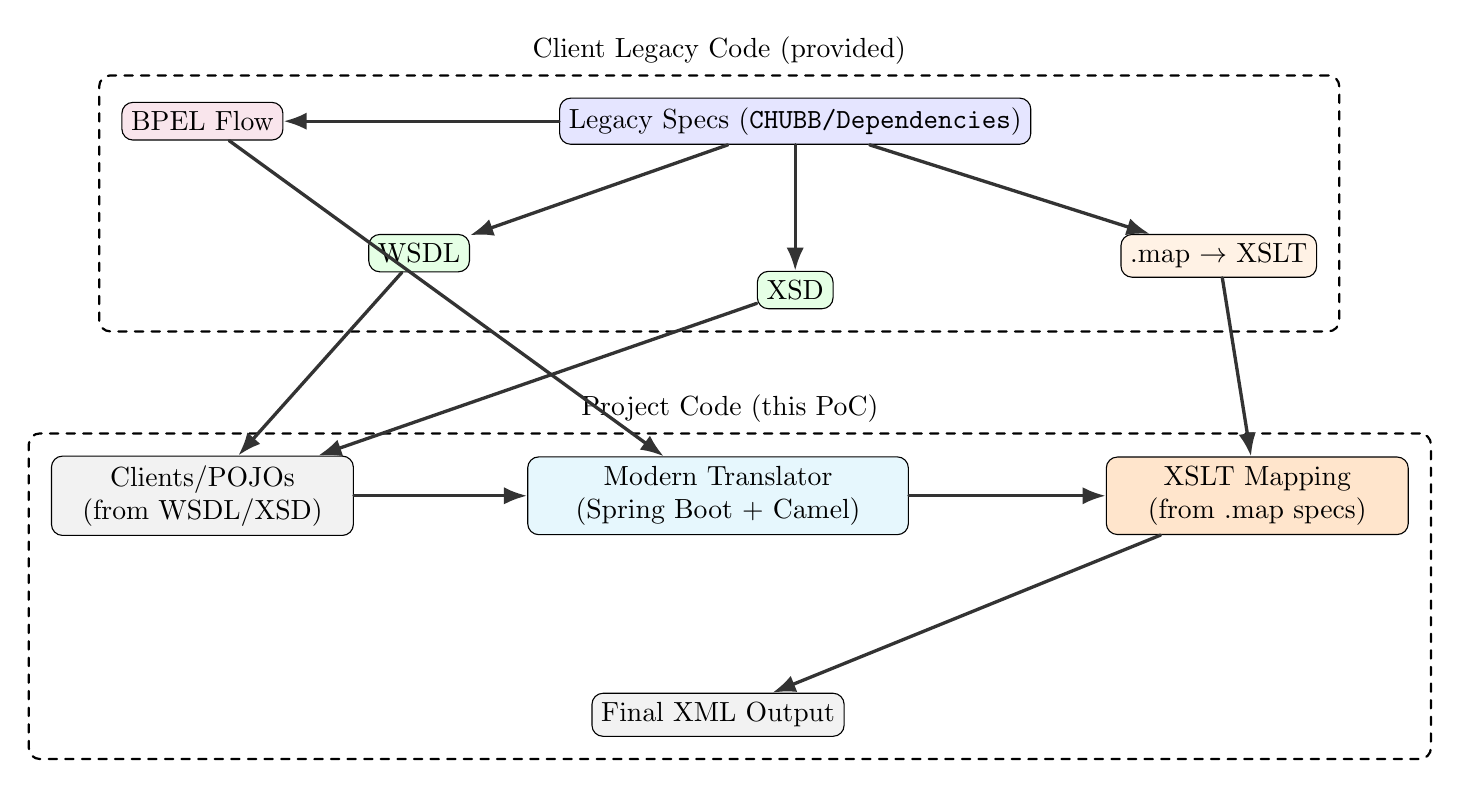
\begin{tikzpicture}[node distance=1.6cm,>=Latex,line cap=round]
  % Legacy specs cluster
  \node (deps2) [draw, rounded corners, fill=blue!10] {Legacy Specs (\texttt{CHUBB/Dependencies})};
  \node (wsdl2) [below left=of deps2, draw, rounded corners, fill=green!10] {WSDL};
  \node (xsd2)  [below=of deps2, draw, rounded corners, fill=green!10] {XSD};
  \node (map2)  [below right=of deps2, draw, rounded corners, fill=orange!10] {.map $\to$ XSLT};
  \node (bpel2) [left=3.5cm of deps2, draw, rounded corners, fill=purple!10] {BPEL Flow};
  % Modern translator
  \node (pojo2) [below=4.0cm of bpel2, draw, rounded corners, fill=gray!10, text width=3.6cm, align=center] {Clients/POJOs\\(from WSDL/XSD)};
  \node (camel) [right=2.2cm of pojo2, draw, rounded corners, fill=cyan!10, text width=4.6cm, align=center] {Modern Translator\\(Spring Boot + Camel)};
  \node (xslt2) [right=2.5cm of camel, draw, rounded corners, fill=orange!20, text width=3.6cm, align=center] {XSLT Mapping\\(from .map specs)};
  \node (xml2)  [below=2.0cm of camel, draw, rounded corners, fill=gray!10] {Final XML Output};
  % Group boxes to separate legacy vs project code
  \node[draw, rounded corners, dashed, thick, fit=(deps2)(wsdl2)(xsd2)(map2)(bpel2), inner sep=8pt, label=above:{Client Legacy Code (provided)}] (legacygrp) {};
  \node[draw, rounded corners, dashed, thick, fit=(camel)(pojo2)(xslt2)(xml2), inner sep=8pt, label=above:{Project Code (this PoC)}] (projgrp) {};
  % Edges
  \draw[flowarrow] (deps2) -- (wsdl2);
  \draw[flowarrow] (deps2) -- (xsd2);
  \draw[flowarrow] (deps2) -- (map2);
  \draw[flowarrow] (deps2) -- (bpel2);
  \draw[flowarrow] (wsdl2) -- (pojo2);
  \draw[flowarrow] (xsd2) -- (pojo2);
  \draw[flowarrow] (bpel2) -- (camel);
  \draw[flowarrow] (pojo2) -- (camel);
  \draw[flowarrow] (map2) -- (xslt2);
  \draw[flowarrow] (camel) -- (xslt2);
  \draw[flowarrow] (xslt2) -- (xml2);
\end{tikzpicture}
\caption{Legacy-to-modern translation pipeline. Client artefacts (top cluster) feed the PoC (bottom cluster): WSDL/XSD drive POJO generation via \texttt{wsdl2java}/\texttt{xjc}; BPEL flow is manually translated into Camel route logic; \texttt{.map} specifications become XSLT stylesheets invoked by the route to transform LOC3X1M responses into LOC3X1B format; final XML is written to \texttt{CHUBB/output/loc3x1\_result.xml} for regression testing.}
\label{fig:translation-pipeline}
\end{figure}



\paragraph{Translation Workflow (Pseudocode)}

Algorithm~\ref{alg:translate-produce} formalises the end-to-end translation and execution process. This is not merely pseudocode for pedagogical purposes—it directly corresponds to the Camel route implementation described in Section~4.

\begin{algorithm}
\caption{Translate and Produce Deterministic Output}
\label{alg:translate-produce}
\begin{algorithmic}[1]
\Function{TranslateAndProduce}{input}
  \State validate(input, XSD)
  \State steps $\gets$ deriveFlowFromBPEL(bpel)
  \ForAll{step in steps}
    \If{step $=$ CRP11X1} \State input $\gets$ callCRP11X1(input) \EndIf
    \If{step $=$ CRP10X1} \State input $\gets$ callCRP10X1(input) \EndIf
    \If{step $=$ LOC3X1M} \State mReply $\gets$ callLOC3X1M(buildMRequest(input)) \EndIf
  \EndFor
  \State mapped $\gets$ applyXSLT(mReply, \texttt{CHUBB/main\_mapper\_with\_submaps.xsl})
  \State mapped $\gets$ applyBusinessRules(mapped) \Comment{e.g., fire district}
  \State writeXML(mapped, \texttt{CHUBB/output/loc3x1\_result.xml})
  \State \Return mapped
\EndFunction
\end{algorithmic}
\end{algorithm}

\noindent\textbf{Detailed algorithmic interpretation}:
\begin{itemize}
  \item \textbf{Line 2 (Validation)}: The input message (e.g., a JSON request from a REST client or an XML document) is validated against the relevant XSD schema. This ensures mandatory fields are present, data types are correct, and cardinality constraints are satisfied. Validation failures abort processing immediately, returning a \texttt{400 Bad Request} or equivalent error. This replicates the BPEL engine's behaviour (Listing~\ref{lst:bpel}, line~4), where invalid input never enters the workflow.

  \item \textbf{Line 3 (Derive flow from BPEL)}: The BPEL file (Listing~\ref{lst:bpel}) is parsed to extract the sequence of operations: enrichment calls (\texttt{CRP11X1}, \texttt{CRP10X1}), the primary service invocation (\texttt{LOC3X1M}), and any conditional branching. In practice, this ``derivation'' is a manual translation performed once during implementation, not a runtime operation. The resulting Camel route hard-codes the sequence: \texttt{.to("direct:crp11x1").to("direct:crp10x1").to("direct:loc3x1m")}.

  \item \textbf{Lines 4--10 (Enrichment loop)}: For each step identified in the BPEL flow, the algorithm conditionally executes enrichment services. \texttt{CRP11X1} (line~5) looks up state/province codes when the input lacks them (e.g., inferring ``CA'' from a ZIP code). \texttt{CRP10X1} (line~7) performs country code enrichment. These services are invoked via SOAP (using generated client stubs from their WSDLs), and their responses augment the \texttt{input} message. This enrichment is critical: downstream services (like \texttt{LOC3X1M}) may require complete address data, and enrichment ensures it's present before invocation.

  \item \textbf{Line 9 (Primary service call)}: \texttt{callLOC3X1M} invokes the core location retrieval service defined in Listing~\ref{lst:wsdl}. The \texttt{buildMRequest} function constructs a \texttt{GetLocationListRequest} object (a JAXB-generated POJO), populating it from the enriched \texttt{input}. The SOAP call returns a \texttt{GetLocationListResponse} (stored in \texttt{mReply}), which contains location data in the LOC3X1M schema format. This step corresponds to Listing~\ref{lst:bpel}, line~5.

  \item \textbf{Line 11 (XSLT mapping)}: The \texttt{mReply} (LOC3X1M format) is transformed into LOC3X1B format using an XSLT stylesheet (\texttt{main\_mapper\_with\_submaps.xsl}). This stylesheet encodes every transformation rule from the client's \texttt{.map} files: field renaming, structural reshaping, default value application, code normalisation. XSLT is deterministic—given the same input, it produces identical output—which is essential for regression testing. The \texttt{applyXSLT} function uses a Java XSLT processor (e.g., \texttt{javax.xml.transform.Transformer}) or Camel's \texttt{.to("xslt:...)")} component.

  \item \textbf{Line 12 (Business rules)}: Additional business logic is applied post-transformation. For example, fire district codes may require special handling: if the \texttt{FireDistrictCode} field is empty but the address falls within a known jurisdiction, a default code is inserted. These rules are too complex or context-dependent to express in XSLT alone, so they're implemented as Java processors or Groovy scripts invoked by the Camel route.

  \item \textbf{Line 13 (Persist output)}: The final \texttt{mapped} XML document is serialised to \texttt{CHUBB/output/loc3x1\_result.xml}. This file serves multiple purposes: (1) it provides a human-readable audit trail, (2) it enables regression testing (comparing current output against golden files), and (3) it can be used for downstream processing or manual review. Writing to disk replicates the BPEL engine's behaviour, where process instances often persist intermediate and final results for observability.

  \vspace{0.5em}
  \noindent\fbox{\parbox{0.95\textwidth}{%
  \textbf{\textcolor{red}{Step 7: Generate services for XML/JSON inputs/outputs}}\\
  \emph{Implemented}: XML output is produced deterministically to \texttt{CHUBB/output/loc3x1\_result.xml}; REST endpoints accept JSON/XML requests and orchestrate the flow.\\
  \emph{Enhance}: Provide content negotiation for responses, validate JSON payloads against a canonical schema, and ensure both XML/JSON outputs align with the same domain model (DTOs) to avoid drift.
  }}
  \vspace{0.5em}

  \item \textbf{Line 14 (Return)}: The function returns the \texttt{mapped} XML, which the Camel route can optionally send to additional endpoints (e.g., a message queue, a REST endpoint, or an archival system).
\end{itemize}

\noindent\emph{Determinism and correctness}: The algorithm's correctness hinges on faithful replication of legacy semantics. If the BPEL process invoked \texttt{CRP11X1} \emph{before} \texttt{LOC3X1M}, we must do the same—reversing the order could yield incorrect results if \texttt{LOC3X1M} expects enriched data. Similarly, the XSLT transformation must implement every mapping rule exactly as specified in the \texttt{.map} files. Any deviation—omitting a field, applying the wrong default, mishandling optionals—constitutes a regression. This is why Algorithm~\ref{alg:translate-produce} emphasises ``translate'' rather than ``rewrite'': we are mechanically converting BPEL steps and \texttt{.map} rules into equivalent Camel/XSLT constructs, preserving behaviour byte-for-byte.

\paragraph{Concrete Example (Real Client Assets)}

To ground the abstract flow in tangible artefacts, we enumerate the actual files from \texttt{CHUBB/Dependencies/} and trace their roles:

\begin{itemize}
  \item \textbf{Contracts}: The \texttt{LocationRetrievalLOC3X1M/} directory contains \texttt{LocationRetrievalLOC3X1M.wsdl} (Listing~\ref{lst:wsdl}), which defines the \texttt{GetLocationList} operation. Bindings specify SOAP 1.2 over HTTP, and the service endpoint URL points to a legacy system (replaced by a mock or test endpoint in the PoC). Messages reference XSD types, ensuring strong typing. Running \texttt{wsdl2java} on this WSDL generates Java classes like \texttt{GetLocationListRequest.java} and \texttt{GetLocationListResponse.java}, which our Camel route instantiates and manipulates \cite{wsdl-spec}.

  \item \textbf{Schemas}: The \texttt{Schemas/} directory houses reusable XSD files: \texttt{StatusInformation.xsd} (Listing~\ref{lst:xsd}), \texttt{TaxingJurisdiction.xsd} (defining tax codes and jurisdiction boundaries), \texttt{TypedAddressX3.xsd} (a complex address structure with optional fields like \texttt{AddressLine3}, \texttt{County}, \texttt{PostalCodeExtension}). These schemas are imported by multiple WSDLs, establishing a shared type library. When code generation runs, types from these schemas become Java classes annotated with JAXB bindings, enabling automatic marshalling and unmarshalling.

  \item \textbf{Orchestration}: \texttt{LocationRetrievalLOC3X1Process.bpel} (Listing~\ref{lst:bpel}) documents the workflow: receive request, enrich with \texttt{CRP11X1} and \texttt{CRP10X1}, invoke \texttt{LOC3X1M}, map to LOC3X1B, reply. In the legacy system, this BPEL process ran on Oracle SOA Suite or IBM Process Server. Our modernisation translates it into a Camel route (\texttt{src/main/resources/camel/main-route.yaml}), using Camel's YAML DSL to express the same sequence of steps \cite{bpel-spec}.

  \item \textbf{Mapping}: \texttt{CHUBB/main\_mapper\_with\_submaps.xsl} is a 500-line XSLT 2.0 stylesheet encoding transformations like ``copy \texttt{LOC3X1M/StatusInformation/StatusCode} to \texttt{LOC3X1B/StatusInformation/StatusCode}, normalising codes (e.g., \texttt{SUCCESS} $\to$ \texttt{0}),'' or ``if \texttt{LOC3X1M/TaxingJurisdiction/FireDistrictCode} is empty, output \texttt{<FireDistrictCode>UNKNOWN</FireDistrictCode>}.'' This stylesheet was generated from \texttt{.map} files (Excel-like specifications maintained by business analysts), ensuring every field-level rule is auditable and version-controlled \cite{xslt-spec}.

  \item \textbf{Execution}: A sample input file, \texttt{CHUBB/sample\_input\_with\_submaps.xml}, provides a representative payload: an address with \texttt{City="Los Angeles"}, \texttt{StateOrProvince="CA"}, \texttt{PostalCode="90210"}, but missing \texttt{Country}. The Camel route processes this input: (1) validates it against \texttt{TypedAddressX3.xsd}, (2) invokes \texttt{CRP10X1} to enrich \texttt{Country="US"}, (3) calls \texttt{LOC3X1M} with the enriched address, receiving a response with location details and tax jurisdiction codes, (4) applies \texttt{main\_mapper\_with\_submaps.xsl} to reshape the response into LOC3X1B format, (5) writes \texttt{CHUBB/output/loc3x1\_result.xml}. This output is then compared (byte-for-byte or semantically) against a golden file to verify correctness.
\end{itemize}

\noindent\emph{Why concrete examples matter}: Abstract descriptions (``we call a service and transform the response'') obscure critical details. By identifying actual files—\texttt{LocationRetrievalLOC3X1M.wsdl}, \texttt{main\_mapper\_with\_submaps.xsl}, \texttt{loc3x1\_result.xml}—we make the workflow tangible. A developer can open these files, trace field mappings line-by-line, and verify that the Camel route implements the intended behaviour. This concreteness is essential for debugging (``the output is missing \texttt{StatusMessage}; let's check if the XSLT handles \texttt{minOccurs="0"} correctly'') and for onboarding new team members (``read \texttt{LocationRetrievalLOC3X1Process.bpel} to understand the workflow, then examine \texttt{main-route.yaml} to see how we translated it'').

\subsection{Modernisation Objectives}

Having understood the legacy artefacts (Section~1.2) and their integration (Section~1.3), we now articulate the modernisation goals. These objectives guide all technical decisions and serve as acceptance criteria for the PoC.

\begin{itemize}
  \item \textbf{Replace legacy orchestration (BPEL, proprietary mappers) with Spring Boot + Apache Camel} \cite{camel-docs}: The client's existing system relies on vendor-specific BPEL engines (Oracle SOA Suite, IBM WebSphere Process Server) and proprietary mapping tools. These platforms incur licensing costs, require specialised skills, and resist modern DevOps practices (e.g., Git-based version control, Docker containerisation, CI/CD pipelines). By re-implementing orchestration in Apache Camel—a vendor-neutral, open-source integration framework—we eliminate vendor lock-in. Camel routes are expressed in YAML or Java DSL, making them readable, testable, and versionable. Spring Boot provides the application runtime, offering autoconfiguration, embedded servers (Tomcat, Jetty), and production-ready features (health checks, metrics, externalised configuration). This combination is cloud-native: the PoC can be packaged as a Docker image, deployed to Kubernetes, and scaled horizontally.

  \item \textbf{Implement data mapping using XSLT and lightweight processors} \cite{xslt-spec}: The client's \texttt{.map} files were authored in proprietary mapping tools (drag-and-drop graphical interfaces). These tools generate artefacts (e.g., Oracle Service Bus \texttt{.xqy} files, IBM \texttt{.mxl} files) that are opaque, difficult to version, and impossible to unit-test in isolation. By translating \texttt{.map} rules into XSLT stylesheets, we gain portability (XSLT processors are ubiquitous), testability (XSLT transformations can be unit-tested with XML input/output fixtures), and transparency (developers can read and modify \texttt{.xsl} files). For transformations too complex for XSLT (e.g., invoking external APIs, applying stateful business rules), we use lightweight Java processors or Groovy scripts within the Camel route. This hybrid approach balances declarative simplicity (XSLT) with procedural expressiveness (Java/Groovy).

  \item \textbf{Integrate enrichment (state/country lookups) and external services using HTTP/SOAP clients} \cite{soap-spec, wsdl-spec}: The legacy workflow invokes multiple external services (\texttt{CRP11X1} for state enrichment, \texttt{CRP10X1} for country enrichment, \texttt{LOC3X1M} for location retrieval). These services expose SOAP interfaces defined by WSDLs in \texttt{Dependencies/}. Our modernisation uses Apache CXF (a JAX-WS implementation) to generate type-safe client stubs from these WSDLs. Camel's \texttt{cxf} component integrates these stubs seamlessly, allowing routes to invoke SOAP services with a single \texttt{.to("cxf:bean:loc3x1mClient")} statement. For services transitioning to REST, Camel's \texttt{http} component provides equivalent functionality. This approach preserves integration contracts (WSDL-defined message formats) whilst enabling gradual migration to modern protocols.

  \item \textbf{Deliver a PoC that writes a verifiable XML artefact to \texttt{CHUBB/output/loc3x1\_result.xml}}: The PoC's success criterion is producing deterministic, correct output. For every sample input (e.g., \texttt{sample\_input\_with\_submaps.xml}), the Camel route must generate an XML file that (1) validates against the LOC3X1B schema, (2) contains all mandatory fields populated correctly, (3) matches the expected output (golden file) byte-for-byte or semantically (ignoring whitespace/comments). This output serves as a regression test baseline: any code change must continue producing identical output for the same input. Writing to a file (\texttt{loc3x1\_result.xml}) provides an audit trail and simplifies comparison (tools like \texttt{xmldiff} or custom validators can assert equivalence). In production, this output would be sent to downstream systems (message queues, databases, REST endpoints), but file-based validation is sufficient for the PoC.
\end{itemize}

\noindent\emph{Why these objectives?} They address the client's pain points: high licensing costs (vendor lock-in), inflexible deployment (monolithic platforms), opaque logic (proprietary mappers), and difficult testing (no CI/CD integration). By targeting open-source, cloud-native technologies, we enable the client to deploy on any infrastructure (AWS, Azure, on-premises Kubernetes), reduce operational costs (no vendor licences), and accelerate development (Git workflows, automated testing, faster iteration). The PoC demonstrates feasibility: ``Can we re-implement this workflow in Camel without changing behaviour?'' If the PoC succeeds, the client gains confidence to modernise additional workflows using the same approach.

\section{Technology Primer}
\subsection{Java and Maven}
Java runs on the JVM and compiles source files into bytecode. Maven is a build tool that manages dependencies, compilation, packaging, and plugins \cite{maven-docs}. The project uses Maven goals like \texttt{compile}, \texttt{package}, and \texttt{spring-boot:run}. 

\subsection{Spring Boot}
Spring Boot simplifies building production-ready services with embedded servers, autoconfiguration, and actuator endpoints \cite{spring-boot}. It provides a clean entry point (\texttt{mainClass}) and integrates seamlessly with Camel. 

\subsection{Apache Camel and YAML DSL}
Apache Camel is an integration framework implementing Enterprise Integration Patterns (EIP). Routes define message flow using components (HTTP, timer, log, etc.). This project uses the YAML DSL to declare routes in \texttt{.yaml} files loaded from the classpath \cite{camel-docs}. 

\subsection{SOAP, WSDL, JAXB, and JAX-WS}
SOAP is an XML-based messaging protocol; WSDL describes service contracts and bindings \cite{soap-spec, wsdl-spec}. JAXB maps XML schemas (XSD) to Java classes (POJOs), while JAX-WS provides SOAP client/server APIs \cite{jaxb-docs, jaxws-docs}. Tools like \texttt{xjc} and \texttt{wsimport}, or Apache CXF \cite{cxf-docs}, generate code from XSD/WSDL. 

\subsection{BPEL}
BPEL (Business Process Execution Language) defines orchestrations of service invocations in XML \cite{bpel-spec}. The client’s BPEL file documents the legacy flow; Camel routes replace its orchestration role in the PoC. 

\subsection{XSLT}
XSLT transforms XML using declarative templates \cite{xslt-spec}. The mapping logic is encoded in \texttt{CHUBB/main\_mapper\_with\_submaps.xsl}, mirroring rules from the client’s \texttt{.map} files. 

\subsection{Supporting Libraries}
MapStruct (compile-time mappers) \cite{mapstruct}, Lombok (boilerplate reduction) \cite{lombok}, Jackson XML (XML binding) \cite{jackson-xml}. These improve productivity without changing core logic.

\section{Client \texttt{Dependencies} Folder}
\subsection{Contents}
\begin{itemize}
  \item Service Contracts: \texttt{LocationRetrievalLOC3X1*/} WSDL/XSD; \texttt{CRP11X1}, \texttt{CRP10X1} WSDL/XSD.
  \item Domain Schemas: \texttt{Schemas/} (e.g., \texttt{StatusInformation.xsd}, \texttt{TaxingJurisdiction.xsd}).
  \item Mapping Specs: \texttt{LOC3X1/*.map} defining request/reply transformations.
  \item Process Doc: \texttt{LocationRetrievalLOC3X1Process.bpel} legacy orchestration.
\end{itemize}

\subsection{Relationship Diagram}
\begin{center}
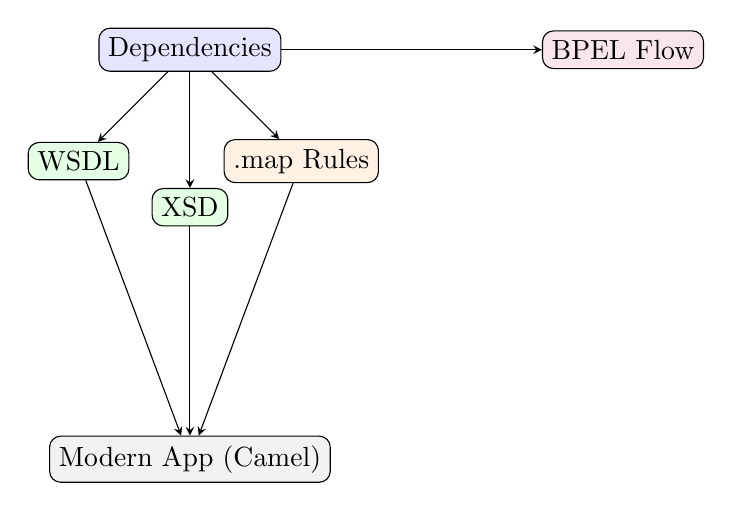
\begin{tikzpicture}[node distance=2.0cm,>=stealth]
  \node (deps) [draw, rounded corners, fill=blue!10] {Dependencies};
  \node (wsdl) [below left of=deps, draw, rounded corners, fill=green!10] {WSDL};
  \node (xsd)  [below of=deps, draw, rounded corners, fill=green!10] {XSD};
  \node (map)  [below right of=deps, draw, rounded corners, fill=orange!10] {.map Rules};
  \node (bpel) [right of=deps, xshift=3.5cm, draw, rounded corners, fill=purple!10] {BPEL Flow};
  \node (app)  [below of=xsd, yshift=-1.2cm, draw, rounded corners, fill=gray!10] {Modern App (Camel)};
  \draw[->] (deps) -- (wsdl);
  \draw[->] (deps) -- (xsd);
  \draw[->] (deps) -- (map);
  \draw[->] (deps) -- (bpel);
  \draw[->] (wsdl) -- (app);
  \draw[->] (xsd) -- (app);
  \draw[->] (map) -- (app);
\end{tikzpicture}
\end{center}

\section{Solution Architecture}
\subsection{Repository Layout}
\begin{itemize}
  \item \texttt{src/main/java}: controllers, services, processors.
  \item \texttt{src/main/resources}: \texttt{application.yml}, Camel routes (YAML), templates.
  \item \texttt{CHUBB/}: XSLT, sample input, output folder, Dependencies (specs).
  \item \texttt{libs/}: external JARs (POJOs, SOAP clients).
\end{itemize}

\subsection{Orchestration Flow}
Camel routes implement validation, enrichment, external calls, and mapping. A simplified flow is shown below.

\begin{center}
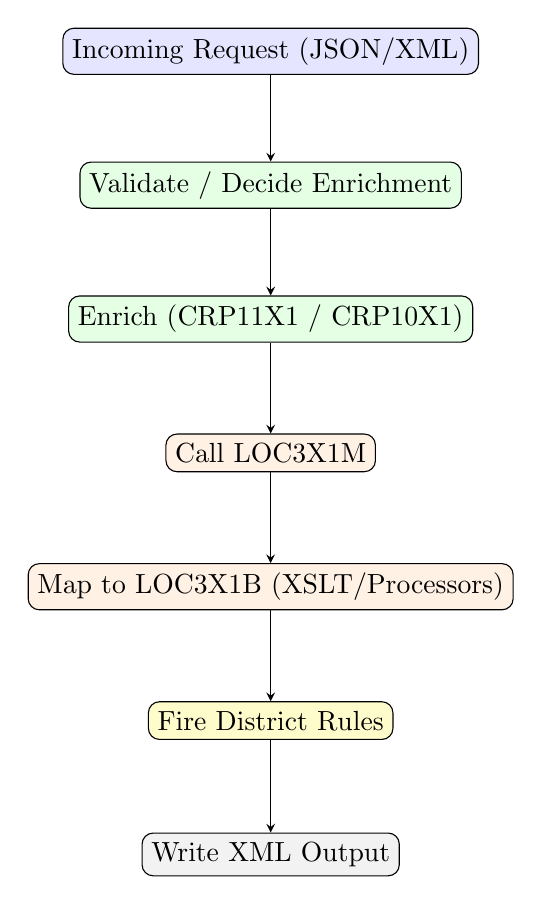
\begin{tikzpicture}[node distance=1.7cm,>=stealth]
  \node (in)   [draw, rounded corners, fill=blue!10] {Incoming Request (JSON/XML)};
  \node (val)  [below of=in, draw, rounded corners, fill=green!10] {Validate / Decide Enrichment};
  \node (enr)  [below of=val, draw, rounded corners, fill=green!10] {Enrich (CRP11X1 / CRP10X1)};
  \node (locm) [below of=enr, draw, rounded corners, fill=orange!10] {Call LOC3X1M};
  \node (map)  [below of=locm, draw, rounded corners, fill=orange!10] {Map to LOC3X1B (XSLT/Processors)};
  \node (fd)   [below of=map, draw, rounded corners, fill=yellow!20] {Fire District Rules};
  \node (out)  [below of=fd, draw, rounded corners, fill=gray!10] {Write XML Output};
  \draw[->] (in) -- (val);
  \draw[->] (val) -- (enr);
  \draw[->] (enr) -- (locm);
  \draw[->] (locm) -- (map);
  \draw[->] (map) -- (fd);
  \draw[->] (fd) -- (out);
\end{tikzpicture}
\end{center}

\subsection{Key Components}
\begin{itemize}
  \item \textbf{Validation Service}: decides if CRP11X1/CRP10X1 lookups are needed.
  \item \textbf{Mapping Service}: orchestrates parsing and XSLT transformation; shapes LOC3X1M reply to LOC3X1B.
  \item \textbf{Processors}: build requests, apply rules (e.g., fire district), convert data structures.
  \item \textbf{XSLT}: implements field-level mapping rules derived from \texttt{.map} specs.
\end{itemize}

\section{Data Mapping: Tables and Pseudocode}
\subsection{Representative Field Mapping}
\begin{center}
\renewcommand{\arraystretch}{1.2}
\begin{tabular}{>{\raggedright}p{0.38\linewidth} >{\raggedright}p{0.38\linewidth} >{\raggedright\arraybackslash}p{0.16\linewidth}}
\toprule
\textbf{Source (RAND/LOC3X1M)} & \textbf{Target (LOC3X1B)} & \textbf{Rule} \\
\midrule
\texttt{StatusInformation/StatusCode} & \texttt{StatusInformation/StatusCode} & Copy, normalize codes \\
\texttt{TaxingJurisdiction/FireDistrictCode} & \texttt{PublicProtection/FireDistrictCode} & Copy, apply defaulting \\
\texttt{Address/StateOrProvince} & \texttt{Address/StateOrProvince} & Enriched via CRP11X1 when missing \\
\texttt{Address/Country} & \texttt{Address/Country} & Enriched via CRP10X1 when missing \\
\texttt{Location/Coordinates} & \texttt{Location/Coordinates} & Copy; validate range \\
\bottomrule
\end{tabular}
\end{center}

\subsection{Pseudocode: Transform Flow}
\begin{algorithm}
\caption{High-level Transform and Orchestration}
\begin{algorithmic}[1]
\Function{ProcessRequest}{input}
  \State validate(input)
  \If{needsStateEnrichment(input)}
    \State input $\gets$ callCRP11X1(input)
  \EndIf
  \If{needsCountryEnrichment(input)}
    \State input $\gets$ callCRP10X1(input)
  \EndIf
  \State loc3x1mReply $\gets$ callLOC3X1M(buildRequest(input))
  \State mapped $\gets$ applyXSLT(loc3x1mReply, main\_mapper\_with\_submaps)
  \State mapped $\gets$ applyFireDistrictRules(mapped)
  \State writeXML(mapped, \texttt{CHUBB/output/loc3x1\_result.xml})
  \State \Return mapped
\EndFunction
\end{algorithmic}
\end{algorithm}


\section{Build and Run}
\subsection{Configuration}
\begin{itemize}
  \item \texttt{application.yml}: enables YAML routes from \texttt{classpath:camel/*.yaml, classpath:*.yaml}; defines service host/port placeholders.
  \item External JARs in \texttt{libs/}: POJOs and SOAP clients referenced via Maven system scope.
\end{itemize}

\subsection{Commands}
\begin{itemize}
  \item Development run: \texttt{mvn -q -DskipTests -Dspring-boot.run.arguments=--server.port=8081 spring-boot:run}
  \item Packaging (optional): \texttt{mvn package}
\end{itemize}

\subsection{Verification}
\begin{itemize}
  \item Demo endpoint triggers the XSLT transformation and writes the output file to \texttt{CHUBB/output/loc3x1\_result.xml}.
  \item Inspect the file to confirm size and content against expectations (e.g., \texttt{happy\_path\_example.xml}).
\end{itemize}

\section{Glossary}
\begin{itemize}
  \item \textbf{WSDL}: XML description of SOAP services (operations, bindings).
  \item \textbf{XSD}: XML Schema Definition, types and constraints.
  \item \textbf{SOAP}: XML-based messaging protocol, often over HTTP.
  \item \textbf{BPEL}: XML language for service orchestration.
  \item \textbf{Camel Route}: Directed flow of message processing steps.
  \item \textbf{XSLT}: Declarative transformation language for XML.
  \item \textbf{POJO}: Plain Old Java Object, simple data holder.
\end{itemize}

\section{Agent-Based Automation with Python, Ollama, and LangGraph}
\subsection{Objective and Scope}
This section evaluates replacing the Java/Camel orchestration with a Python implementation that preserves deterministic mapping while introducing deep-agent capabilities for assistive tasks. The proposed stack uses a local LLM via Ollama \cite{ollama-docs}, a graph-based workflow engine via LangGraph \cite{langgraph-docs}, and a FastAPI service layer \cite{fastapi-docs}. Deterministic XML transforms remain in XSLT using \texttt{lxml} \cite{lxml-docs}, and SOAP integration is handled by \texttt{zeep} \cite{zeep-docs}.

\subsection{Feasibility and Constraints}
\begin{itemize}
  \item \textbf{Realizable}: All current stages (validate, enrich, external call, map, rules, persist) have Python equivalents.
  \item \textbf{Determinism}: Field-level transforms remain in XSLT; agents provide non-authoritative assistance (QA, normalization, suggestions).
  \item \textbf{Parities}: A golden-file test suite must prove Python outputs equal to the Java implementation for representative inputs.
\end{itemize}

\subsection{Architecture Overview}
\begin{itemize}
  \item \textbf{Service Layer}: FastAPI endpoints mirror current REST surfaces.
  \item \textbf{Workflow}: LangGraph nodes for validation, enrichment (CRP11X1/CRP10X1), LOC3X1M call, XSLT mapping, rule application, persistence.
  \item \textbf{Agents}: Ollama-backed nodes augment input hygiene and anomaly detection, logging explainable recommendations without mutating canonical data.
  \item \textbf{Integration}: \texttt{zeep} consumes WSDLs from \texttt{Dependencies} to invoke SOAP services; \texttt{lxml.etree.XSLT} runs \texttt{main\_mapper\_with\_submaps.xsl}.
\end{itemize}

\subsection{Workflow (Pseudocode)}
\begin{algorithm}
\caption{Python Orchestration with Deterministic Mapping}
\begin{algorithmic}[1]
\Function{ProcessRequestPython}{input}
  \State validate(input) \Comment{deterministic checks}
  \If{needsStateEnrichment(input)}
    \State input $\gets$ callCRP11X1(input) \Comment{zeep/WSDL}
  \EndIf
  \If{needsCountryEnrichment(input)}
    \State input $\gets$ callCRP10X1(input) \Comment{zeep/WSDL}
  \EndIf
  \State loc3x1mReply $\gets$ callLOC3X1M(buildRequest(input))
  \State mapped $\gets$ applyXSLT(loc3x1mReply, main\_mapper\_with\_submaps) \Comment{lxml.XSLT}
  \State mapped $\gets$ applyFireDistrictRules(mapped) \Comment{explicit rules}
  \State agentQA $\gets$ ollamaQA(mapped) \Comment{non-authoritative, logged}
  \State writeXML(mapped, \texttt{CHUBB/output/loc3x1\_result.xml})
  \State \Return mapped
\EndFunction
\end{algorithmic}
\end{algorithm}

\subsection{Migration Plan}
\begin{itemize}
  \item \textbf{Baseline}: Export current Java outputs for multiple inputs as golden files.
  \item \textbf{Deterministic Core}: Implement FastAPI + LangGraph nodes; wire zeep calls and XSLT mapping first.
  \item \textbf{Agent Augmentation}: Add Ollama nodes for QA and normalization that produce logs and operator guidance.
  \item \textbf{Parity Tests}: Require byte-equivalent or schema-equivalent outputs against golden files.
  \item \textbf{Rollout}: Expose identical endpoints; run side-by-side until confidence is achieved.
\end{itemize}

\subsection{Pros and Cons}
\begin{itemize}
  \item \textbf{Pros}: Deterministic transforms preserved; local LLM (privacy); graph workflows are testable and maintainable.
  \item \textbf{Cons}: Added effort to reimplement SOAP bindings; LLM outputs are non-deterministic and must be scoped to assistive roles.
\end{itemize}

\subsection{Conclusion}
A Python + LangGraph + Ollama approach is feasible when deterministic mapping stays in XSLT, agents are constrained to advisory functions, and parity testing governs acceptance. This yields a maintainable, auditable system with optional intelligent QA.

\section{References}
\bibliographystyle{plain}
\bibliography{references}

\end{document}